\subsection{Unlocking the Secrets of Shielded Cables!}

% Question ID
\begin{tcolorbox}[colback=gray!10, colframe=black, title=E4E07] 

% Question Text
Which of the following can cause shielded cables to radiate or receive interference?

% Choices
\begin{enumerate}[label=\Alph*.]
    \item Low inductance ground connections at both ends of the shield
    \item \textbf{Common-mode currents on the shield and conductors}
    \item Use of braided shielding material
    \item Tying all ground connections to a common point resulting in differential-mode currents in the shield
\end{enumerate} \end{tcolorbox}

% Explanation of Concepts
In radio communication and electronics, shielded cables are designed to minimize electromagnetic interference (EMI) from external sources and to prevent signal leakage from the cable itself. However, there are several factors that can lead to unwanted interference, which is critical to understand for effective communication system design.

One significant cause of interference in shielded cables is common-mode currents. These occur when there is a potential difference between the ground reference at the transmitting and receiving ends, causing unwanted currents to flow along the shield and potentially affecting the signal carried by the cable. 

In contrast, low inductance ground connections typically enhance the performance of shielded cables by minimizing the ground loop interference. Although using braided shielding material generally provides better shielding effectiveness, it can still be compromised by improper grounding or layout.

Additionally, tying all ground connections to a common point can lead to differential-mode currents, which although may help in some cases, can also create issues if not managed properly. 

In summary, common-mode currents on the shield and conductors (option B) are a crucial aspect that can lead to interference in shielded cables.

% Diagram (if needed)
\begin{center}
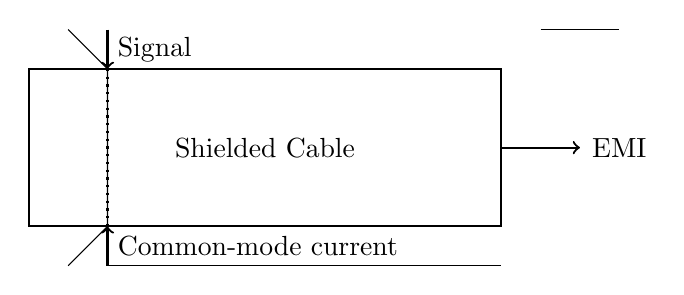
\begin{tikzpicture}
    \draw[thick] (0,0) rectangle (6,2);
    \node at (3,1) {Shielded Cable};
    \draw[->, thick] (6,1) -- (7,1);
    \node at (7.5,1) {EMI};
    
    \draw[thick, ->] (1,2.5) -- (1,2) node[midway, right] {Signal};
    \draw[thick, ->] (1,-0.5) -- (1,0) node[midway, right] {Common-mode current};
    
    \draw[thick, dotted] (1,2) -- (1,-0.5);
    \draw (0.5, 2.5) -- (1,2) -- (1,0) -- (0.5,-0.5);
    \draw (1,-0.5) -- (6,-0.5);
    \draw (6.5,2.5) -- (7.5,2.5);
\end{tikzpicture}
\end{center}
